%to Run the tex file use the command: xelatex  --shell-escape Sample_poster_FA.tex
\documentclass[a0,portrait]{a0poster}
\usepackage{multicol} % This is so we can have multiple columns of text side-by-side
\columnsep=100pt % This is the amount of white space between the columns in the poster
\columnseprule=3pt % This is the thickness of the black line between the columns in the poster

\usepackage[svgnames]{xcolor} % Specify colors by their 'svgnames', for a full list of all colors available see here: http://www.latextemplates.com/svgnames-colors

\usepackage{times} % Use the times font
%\usepackage{palatino} % Uncomment to use the Palatino font
%\usepackage{subfig}

\usepackage{graphicx} % Required for including images
\graphicspath{{figures/}} % Location of the graphics files
\usepackage{booktabs} % Top and bottom rules for table
\usepackage[font=small,labelfont=bf]{caption} % Required for specifying captions to tables and figures
\usepackage{amsfonts, amsmath, amsthm, amssymb} % For math fonts, symbols and environments
\usepackage{wrapfig} % Allows wrapping text around tables and figures
\usepackage[pages=some]{background}
\backgroundsetup{
scale=1.05,
color=black,
opacity=0.15,
angle=0,
contents={%
  \centering 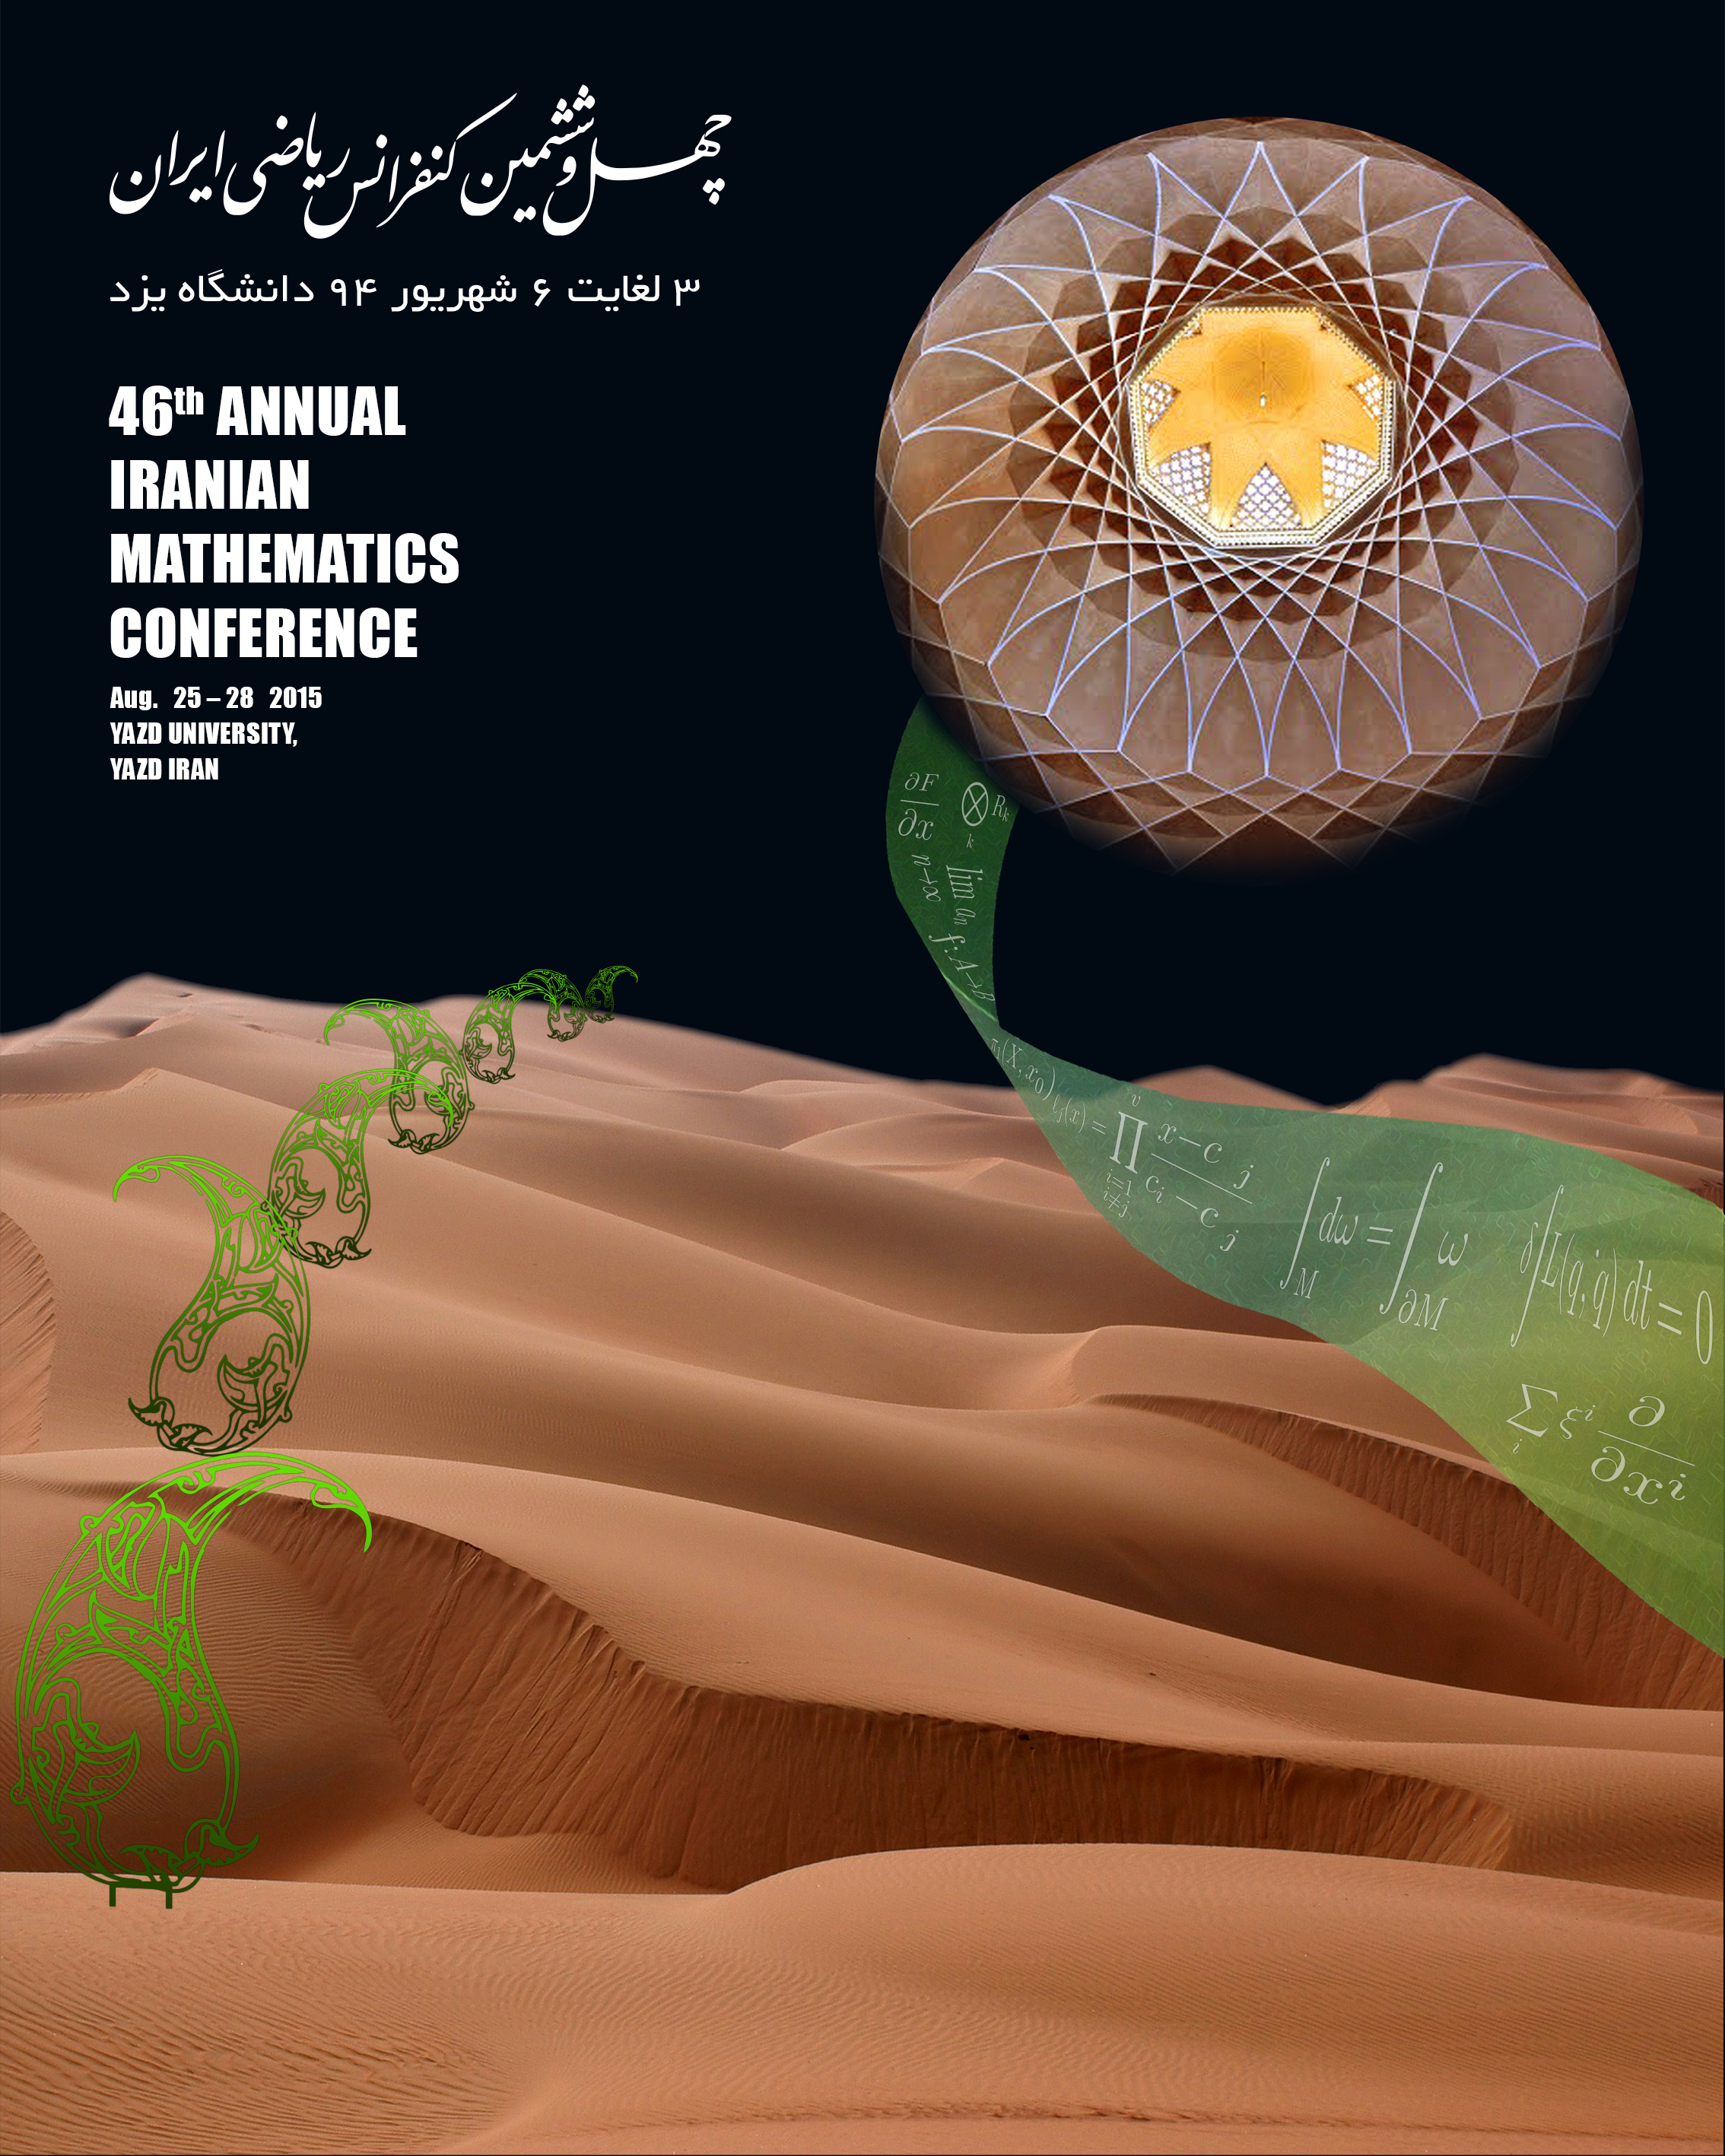
\includegraphics[width=\paperwidth,height=\paperheight]{poster.jpg}
  }%
}

\usepackage{xepersian}
\settextfont[BoldFont={YasBd.ttf},ItalicFont={YasIt.ttf},BoldItalicFont={YasBdIt.ttf}]{YasBd.ttf}
%\setlatintextfont{Times New Roman}
\setdigitfont{Yas.ttf}
\theoremstyle{definition}
\newtheorem{definition}{تعریف}[section]
\theoremstyle{plain}
\newtheorem{theorem}[definition]{قضیه}
\newtheorem{lemma}[definition]{لم}
\newtheorem{proposition}[definition]{گزاره}
\newtheorem{corollary}[definition]{نتیجه}
\theoremstyle{definition}
\newtheorem{example}[definition]{مثال}
\newtheorem{remark}[definition]{ملاحظه}
\newtheorem*{solution}{حل}
\def\OO{\mathcal{O}}
\newcommand{\comment}[1]{}
\newcommand{\keywords}[1]{}
\newcommand{\subject}[1]{}

\begin{document}

 \BgThispage
\begin{center}
\VERYHuge \textbf{مرتب‌سازی زوج نقاط بر مبنای فاصله آن‌ها}\\  %Title
\huge \textbf{محمد فرشی و ابوالفضل پورعیدی و ذریه سلطانی}\\[0.5cm] % Author(s)
\large آزمایشگاه تحقیقاتی الگوریتم‌های ترکیبیاتی و هندسی، گروه علوم کامپیوتر، دانشکده ریاضی، دانشگاه یزد\\[0.4cm] % University/organization
\large \texttt{mfarshi@yazd.ac.ir} و  \texttt{a.poureidi@GMail.com}  و \texttt{z.soltani88@GMail.com}--- 52254%\\ %کد رهگیری
\end{center}

\vspace{1cm} % A bit of extra whitespace between the header and poster content

%----------------------------------------------------------------------------------------

\begin{multicols}{2} % This is how many columns your poster will be broken into, a portrait poster is generally split into 2 columns


%\large


\begin{abstract}\normalsize
مرتب‌سازی داده‌ها یکی از مسائل اساسی و اولیه در علوم کامپیوتر است که مطالعه وسیعی روی آن انجام شده
است و مسائل بسیاری از آن استفاده می‌کنند. در بسیاری از مسائل که روی داده‌های هندسی نظیر مسائل روی نقاط و خطوط در صفحه یا
فضای اقلیدسی با ابعاد بالاتر کار می‌کنند، مساله مرتب‌سازی زوج نقاط بر مبنای
فاصله بین آنها مطرح می‌شود. با به کار بردن الگوریتم‌های معمول برای مرتب‌سازی
داده‌ها، می‌توان برای هر $n$ نقطه، $n\choose 2$ زوج نقطه را بر مبنای 
فاصله بین آنها در زمان $\OO(n^2\log n)$ مرتب کرد.  البته برای
$\Theta(n^2)$ داده مستقل، این مساله راه حل سریع‌تری ندارد ولی با توجه به وابستگی
اعداد در این حالت، موضوع امکان حل این مساله در زمان کمتر و یا داشتن همین کران پایین
جالب به نظر می‌رسد.
در این مقاله به این موضوع می‌پردازیم که آیا می‌توان این مساله را در زمان کمتری
حل کرد یا این مساله دارای کران پایین $\Omega(n^2\log n)$ است.
\end{abstract}
\keywords{مرتب‌سازی، فاصله‌ها، فضای اقلیدسی، کران پایین، پیچیدگی.}
\subject{68Q25, 68Q17}


\section{مقدمه}
مساله مرتب‌سازی داده‌ها یکی از مسائل اساسی مطرح شده در علوم کامپیوتر است که نتایج کاملی از پیچیدگی انجام آن و همچنین الگوریتم‌های بهینه متعددی برای حل آن ارائه شده است. این مساله، در حل سایر مسائل نیز استفاده فراوانی دارد و هر نتیجه در این مساله مستقیماً به سایر مسائلی که از آن استفاده می‌کنند تاثیر می‌گذارد. مسائل پایه‌ای مانند جستجو، یافتن نزدیک‌ترین جفت نقاط، ساخت درخت پوشای کمینه، ساخت اشکال محدب بهینه (شامل تمام نقاط با کمترین مساحت)، انتخاب اعداد با مرتبۀ مشخص از نظر بزرگی در یک مجموعه (مثلاً چهارمین بزرگترین عدد)  که خود در کاربردهای بزرگتری همچون پیاده‌سازی موتورهای جستجوگر، ایجاد نقشه‌ی راه‌ها، کنترل ترافیک هوایی، گرافیک کامپیوتری، رباتیک مورد استفاده قرار می‌گیرند، همگی از الگوریتم‌های مرتب‌سازی اعداد استفاده می‌نمایند. 

همان طور که می‌دانیم در حالت کلی تمام الگوریتم‌های (مقایسه محور) مطرح شده‌ برای مرتب‌سازی 
$\Theta(n)$ عدد،  و دارای کران پایین $\Omega(n\log n)$ هستند و از طرفی پیچیدگی زمانی بسیاری از الگوریتم‌هایی که خود در زمانی کمتر از این کران انجام می‌شوند به دلیل نیاز به مرتب‌سازی داده‌هایشان بر اساس این کران تعیین می‌شود. از این جمله می‌توان به الگوریتم حریصانه برای ساخت پوشش‌های هندسی اشاره کرد \cite{ns-gsn-07}. نکتۀ قابل تأمل در تعدادی از این مسائل این است که آن‌ها به مرتب‌سازی اعدادی نیاز دارند که این اعداد همان فاصله‌های بین جفت نقاط در صفحه هستند. لذا، کران پایین ارائه شده برای مسالۀ مرتب‌سازی، برای مرتب‌سازی فاصله‌ها قابل استفاده نیست. 
بنابراین در ادامه مسأله جدیدی  مطرح می‌شود که در این مقاله برای یافتن راه حلی برای آن تلاش شده است.
البته، در این مقاله به این سوال، پاسخی داده نخواهد شد، بلکه روشی برای بررسی مساله ارائه می‌شود که امید است با تکمیل آن، بتوان این مساله را حل نمود. 

{\bf تعریف مسئله:} مجموعه $S=\{p_1,p_2,\ldots,p_n\}\subset \mathbb{R}^d$
شامل $n$ نقطه %از $\mathbb{R}^d$ 
داده شده است. 
 هدف مرتب کردن تمام زوج نقاط $(p_i,p_j)$ از نقاط $S$  به ترتیب
صعودی بر مبنای فاصله بین نقاط است. 

با توجه به الگوریتم‌های موجود به راحتی می‌توان این زوج‌ها را در زمان 
$\OO(n^2\log n)$ مرتب کرد (تعداد زوج نقاط $\Theta(n^2)$ است). 
البته در حالت کلی نیز مرتب‌سازی 
$\Theta(n^2)$ عدد دارای کران پایین $\Omega(n^2\log n)$ است 
اما در این مسأله،  اعداد ورودی دارای 
این خاصیت اضافی هستند که هر کدام متناظر با فاصله بین دو نقطه در
 $\mathbb{R}^d$
 هستند. 
سوال این است که آیا در این مسأله می‌توان زوج نقاط را در زمان $o(n^2\log n)$ 
مرتب کرد یا این مساله نیز دارای کران پایین مسالۀ مرتب‌سازی است؟

در این مقاله، این مساله را در ساده‌ترین حالت، یعنی وقتی نقاط از فضای 
$\mathbb{R}$
انتخاب شده باشند، بررسی می‌شود.

\section{درخت تصمیم مرتب‌سازی  فاصله‌ها }
برای یافتن کران پایین زمان مرتب‌سازی  $n\choose 2$ فاصله متمایز، 
یک روش، مشابه روش ارائه شده برای یافتن کران پایین برای مسالۀ مرتب‌سازی  
$n$ نقطه است (فصل هشت از کتاب \cite{clrs-ia-09} را ببینید). 
در این روش،  تعداد کل جایگشت‌های ممکن برای مرتب‌سازی 
 $n \choose 2$ فاصله تولید شده توسط $n$ نقطه روی
 خط  حقیقی  را محاسبه و سپس روی آنها یک درخت تصمیم می‌سازیم
 که عمق این درخت تصمیم، کران پایین مساله  را مشخص می‌کند.  مشکل اساسی در ساخت این
 درخت تصمیم این است که با توجه به وابستگی اعداد حاصل از فاصله بین زوج نقاط، بسیاری از 
 مقایسه‌ها که در داده‌های مستقل مورد نیاز است، در این حالت مورد نیاز نیست. این عدم نیاز، در صورتی که به تعداد زیادی مقایسه برسد، می‌تواند این مساله را به یک مساله قابل حل در زمان $\OO(n^2)$ تبدیل
 کند و در غیر این صورت، کران پایین $\Omega(n^2\log n)$ را برای این مساله ثابت کند.

 \subsection{ساخت درخت تصمیم}

 در ساختن یک درخت تصمیم برای مرتب‌سازی $n$ عدد، عملاً به درختی
 می‌رسیم که هر برگ آن متناظر با جایگشتی از اعداد ورودی است که با آن جایگشت،
 اعداد ورودی مرتب هستند. در صورت  مستقل بودن اعداد، هر جایگشت از اعداد  ورودی
 در یک برگ درخت تصمیم باید ظاهر شود. این موضوع در مرتب‌سازی فاصله‌ها
 متفاوت است زیرا بین فاصله‌ها وابستگی وجود دارد و ممکن است برخی از 
 جایگشت‌های $n\choose 2$، اصلاً اتفاق نیفتد و لذا این جایگشت‌ها لازم نیست
 در برگ‌های درخت تصمیم ظاهر شود. در این بخش به محدود کردن این جایگشت‌ها
 می‌پردازیم. 
 
 برای ساخت این درخت ابتدا لازم است ماتریس فاصله‌های بین نقاط و 
 خواص این ماتریس بیان شوند. این ماتریس به ما کمک می‌کند تا از مقایسه‌های 
 غیرضروری هنگام مرتب‌سازی  فاصله‌ها اجتناب کنیم و تنها مقایسه‌هایی که نیاز 
 هستند، انجام شود. فرض کنید همان‌طور که قبلا بیان شد، $n$ نقطه 
 $p_1,p_2,\ldots,p_n$ به ترتیب از چپ به راست روی یک خط دلخواه داریم.
 به وضوح به ازای هر $i$، فاصله $p_i$ تا نقاط بعد از آن به همان ترتیب
 قرار گرفتن نقاط بعد از $p_i$ است. به عبارت دیگر، به ازای هر $i$ داریم:
 $|p_ip_{i+1}|< |p_ip_{i+2}|<\cdots <|p_ip_n|$.
ماتریس فاصله‌ی $D=(d_{i,j})_{n\times n}$ شامل
 فاصله‌ی بین تمام زوج نقاط ‎$d_{i,j}=|p_{i}p_{j}|$
تعریف می‌شود.
‏این ماتریس به وضوح نسبت به قطر اصلی متقارن است و تمام
درایه‌های قطر اصلی صفر است. 
لذا فقط مرتب‌سازی عناصر بالای قطر اصلی ماتریس $D$ مورد نظر است و 
از این به بعد تنها این عناصر را درنظر گرفته و مورد بحث قرار می دهیم. 
با توجه به این که نقاط روی خط قرار دارند، ماتریس $D$  دارای خواص زیر است:
اولاً عناصر هر سطر در حرکت از سمت چپ به سمت راست صعودی هستند و ثانیاً عناصر هر ستون از بالا به پایین نزولی هستند.

 لذا در مرتب‌سازی، نیاز به بررسی زوج نقاطی که 
 ترتیب آنها بر این مبنا مشخص است، نیست. هرچند 
 در قسمت \ref{note-prblms} خواهیم دید که بخش زیادی از مقایسه‌های 
 غیرضروری را این خاصیت صدق می‌کند ولی همۀ آنها در این خاصیت
 صدق نمی‌کنند. 

با توجه به خاصیت اول ماتریس $D$،
کوچک‌ترین درایۀ  ماتریس،  یک درایه از عناصر روی قطر بلافاصله بعد از قطر اصلی ماتریس است.
 نکته بسیار مهم این است که با توجه به دو خاصیت ماتریس، هر درایه
 در صورتی می‌تواند به عنوان کوچک‌‌ترین درایۀ  بعدی در مرتب‌سازی صعودی 
 فاصله‌ها ‌انتخاب شود که در حال حاضر درایۀ انتخاب نشده‌ای 
  در سمت چپ و در پایین آن درایه نباشد.
  
 لذا در هر مرحله، عنصری می‌تواند به عنوان کوچک‌ترین بعدی انتخاب شود که
 سمت چپ و پایین آن خالی باشد، یعنی قبلاً در روند مرتب‌سازی برداشته شده باشند.
پس برای انتخاب کوچکترین عنصر (عنصر اول لیست مرتب شده) 
$n-1$ انتخاب داریم. پس از انتخاب آن برای کوچک‌ترین بعدی 
(عنصر دوم لیست مرتب شده) بسته به اینکه عنصر دوم در کجاست، 
سطر مجاور به سطر عنصر اول یا سطر غیر مجاور به آن،
 به ترتیب $n-1$ یا $n-2$ انتخاب خواهیم داشت.

ما این روند انتخاب و تعداد امکان‌های ممکن برای انتخاب عناصر را در قالب
 ساختار درخت تصمیمی که شرح داده خواهد شد بیان می‌کنیم. 
 مشابه روش اثبات کران پایین برای زمان اجرای مساله مرتب‌سازی اعداد، 
 درخت تصمیم را متناظر با هر شکل اجرای الگوریتم تشکیل می‌دهیم. 
 برگ‌های درخت، متناظر با تمام جایگشت‌هایی است که ممکن است در
 مرتب‌سازی فاصله‌ها رخ دهد.
بوضوح، تمام جایگشت‌های روی $d_{i,j}$ها معتبر نیست.
 به عنوان مثال جایگشتی که $d_{1,3}$ قبل از
$d_{1,2}$ قرار گیرد اتفاق نمی‌افتد.
 
بر مبنای نکته کلیدی بیان شده در بالا، درخت به صورت زیر ساخته می‌شود:

 در ریشه، باید کوتاه‌ترین فاصله (کوچک‌ترین درایۀ ماتریس) قرار گیرد. 
 همانطور که دیدیم این 
عنصر می‌تواند هر درایۀ بلافاصله بعد از  قطر اصلی ماتریس $D$  باشد. فرض کنید
امکان انتخاب عناصر روی این قطر از بالا به پایین به ترتیب به فرزندان ریشه از
 سمت راست به چپ نظیر شوند. لذا درجه ریشه $n-1$ است.
این درخت $n\times(n-1)/2$ سطح دارد که در هر سطح یک عنصر 
لیست مرتب شده مشخص می‌شود: در سطح $i$ام درخت، $i$امین کوچک‌ترین عنصر ماتریس مشخص 
شده و از ماتریس حذف شده به لیست مرتب شده اضافه می‌شود.
این درخت برای $4$ نقطه در روی خط و تمام جایگشت‌های ممکن برای مرتب‌سازی 
صعودی $6$ فاصله متمایز حاصل از این چهار نقطه در
 شکل~\ref{fig-DesTree} شده است:
%\begin{figure}[htb]
\begin{center}\vspace{1cm}
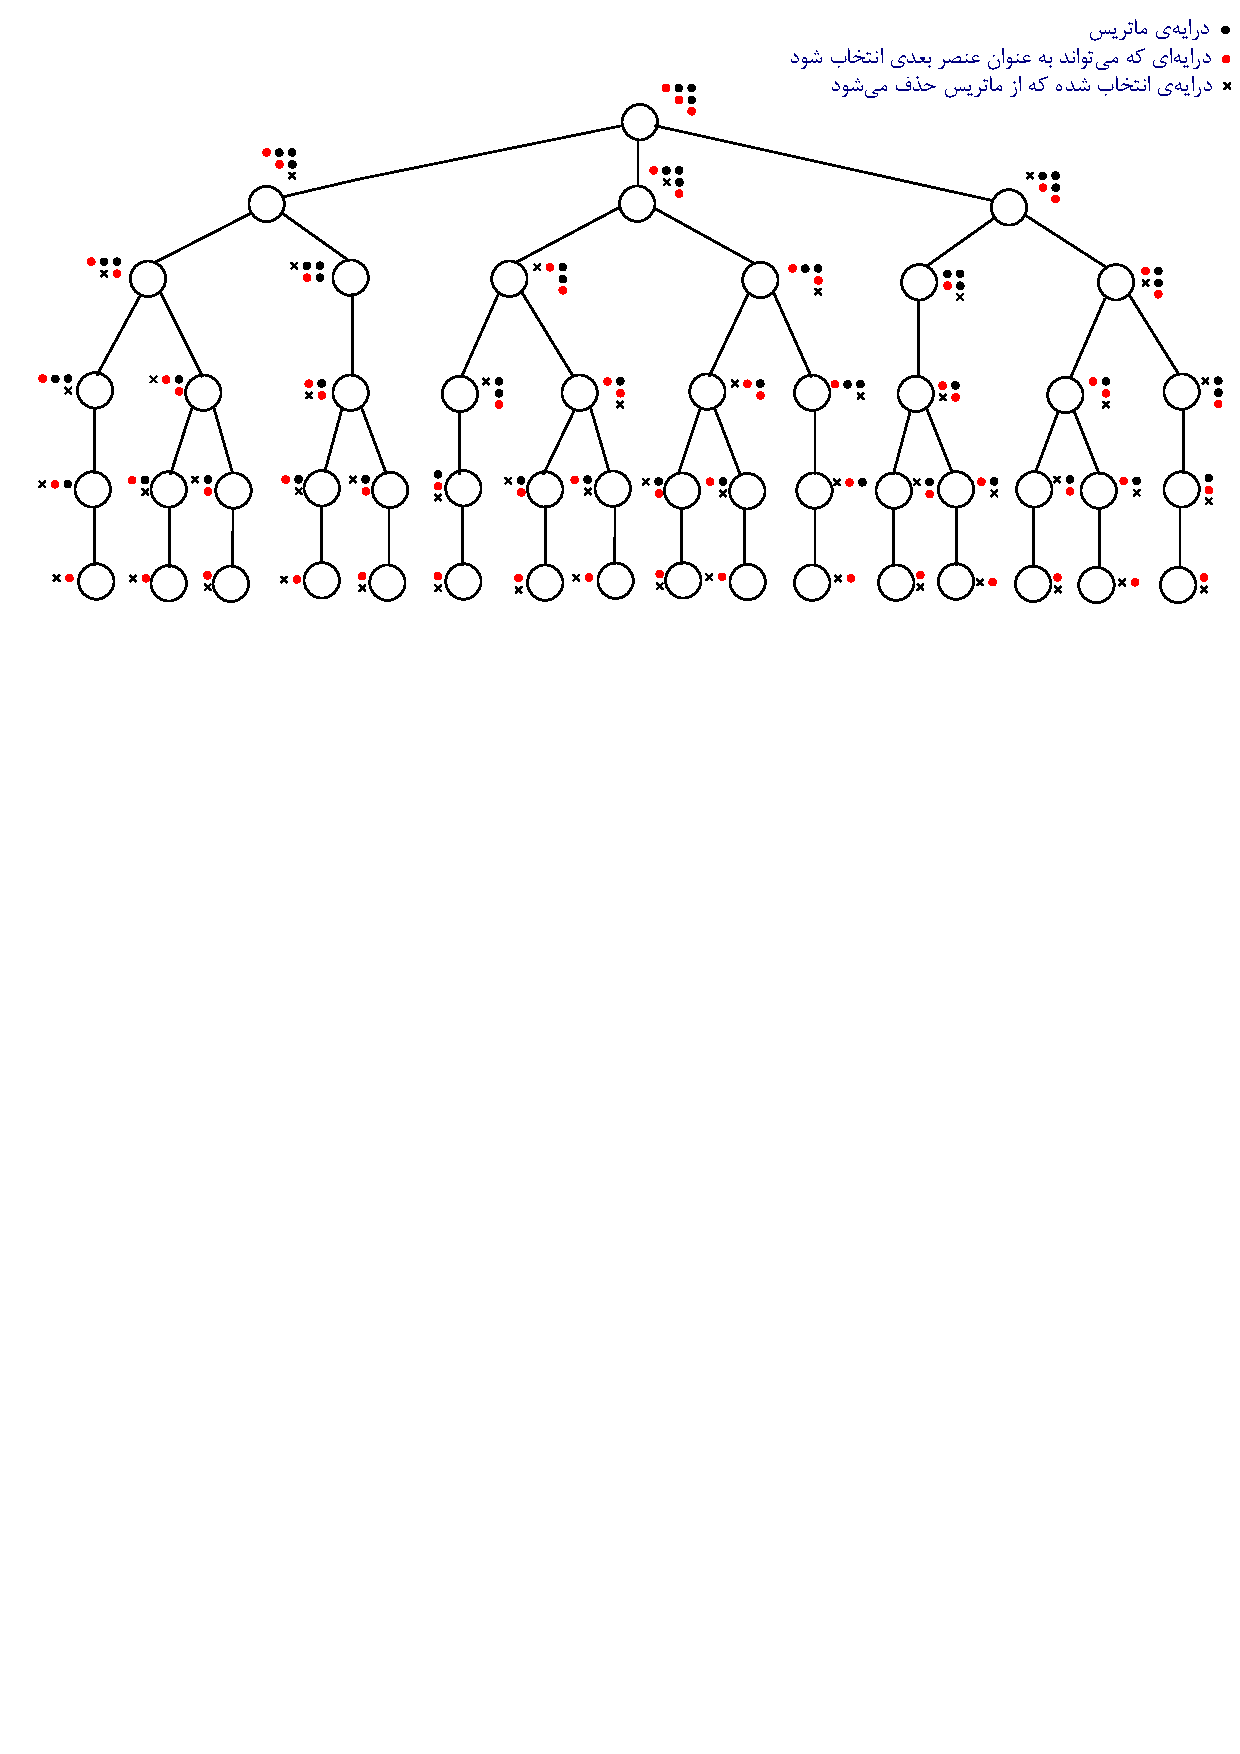
\includegraphics[width=0.48\textwidth]{DesTree.pdf}
\captionof{figure}{درخت تصمیم مرتب‌سازی ۶ فاصله‌ی حاصل از ۴ نقطه روی خط.}
\label{fig-DesTree}
\end{center}
%\end{figure}
پس از معرفی این درخت، که آن را درخت تصمیم مرتب‌سازی فاصله‌ها می‌نامیم، 
مشخص است که این درخت تمام جایگشت‌های ممکن برای مرتب‌سازی را ایجاد 
می‌کند، هرچند تمام این مقایسه‌ها ضروری نیست.
در ابتدا تصور می‌شد که برگ‌های این درخت برابر است با تعداد دقیق 
 جایگشت‌های معتبری که در آن‌ها هیچ مقایسه‌ی غیرضروری صورت نمی‌گیرد، 
 اما همچنان که در شکل~\ref{fig-prlm-sort} آمده، برای مرتب‌سازی چهار نقطه روی
 خط، با انجام مقایسه‌ی $d_{34}<d_{12}$ این نتیجه‌ی بدیهی 
 حاصل می‌شود که $d_{24}<d_{13}$  است و بنابراین دیگر نیازی 
 به انجام این مقایسه در سطح‌های پایین ‌تر درخت نیست و لذا 
 شاخه قرمز رنگ در مسیر 
 مشخص شده دیگر نیاز نیست و باید حذف شود. 

%\begin{figure}[htb]
\begin{center}\vspace{1cm}
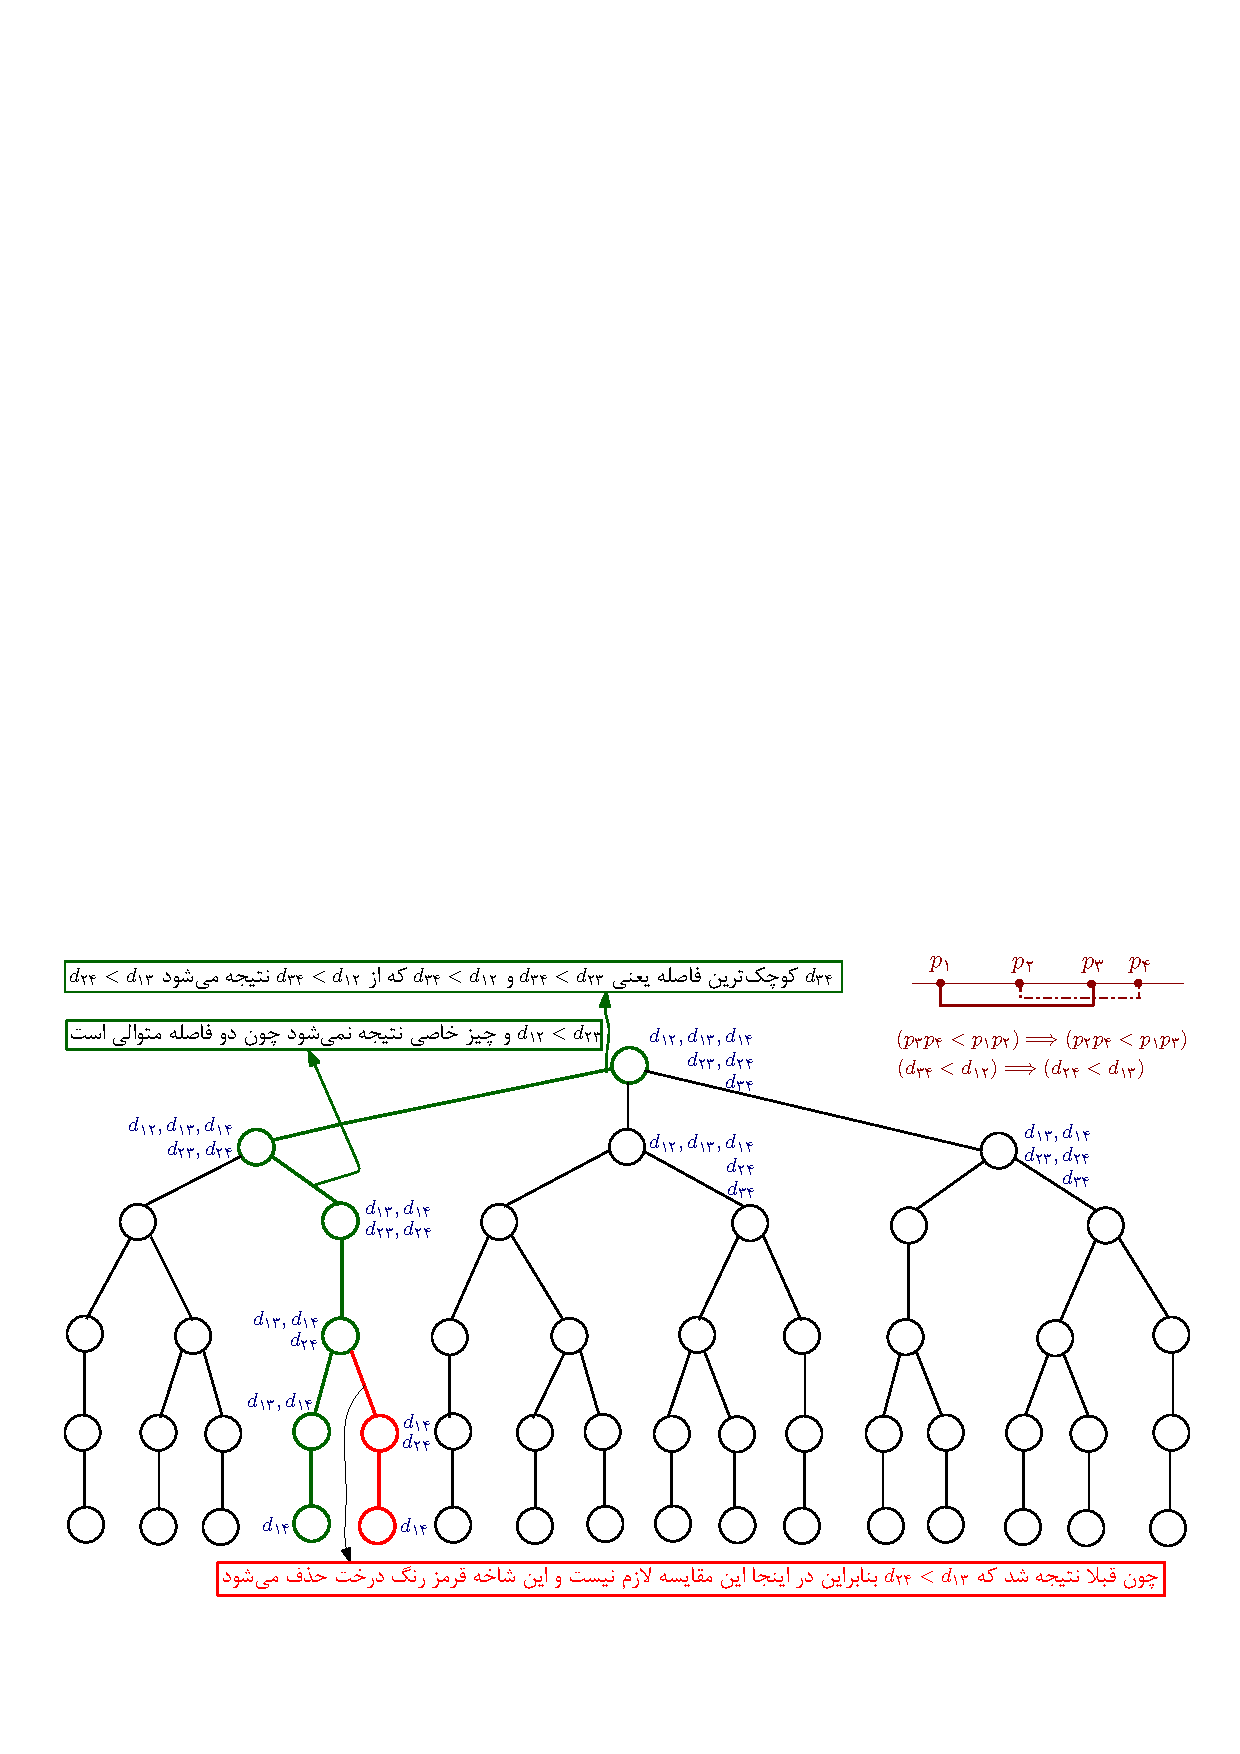
\includegraphics[width=0.48\textwidth]{prblmOnSort.pdf}
\captionof{figure}{یک مسیر اضافی در درخت تصمیم که به یک جایگشت معتبر منجر نمی‌شود.}
\label{fig-prlm-sort}
\end{center}
%\end{figure}	
\section{نتیجه‌گیری و  کارهای آینده} \label{note-prblms}
 در این مقاله سعی شد در خصوص پیچیدگی مقایسۀ فاصلۀ بین $n$ نقطه روی خط حقیقی نتیجه‌ای بدست آید. هرچند این مهم حاصل نشد ولی به نظر می‌رسد ادامه همین روند با حذف جایگشت‌های غیر ضروری از درخت تصمیم و در نهایت شمارش تعداد برگ‌های درخت حاصل، بتوان برای پیچیدگی مساله کرانی بدست آورد. اگر این تعداد به اندازه کافی بزرگ باشد (یعنی از $\Omega(n^{n^2})$) باشد، آنگاه نتیجه خواهد شد که مساله دارای کران پایین $\Omega(n^2\log n)$ است و  در صورت کمتر بودن تعداد برگ‌ها، این امید حاصل می‌شود که الگوریتمی با پیچیدگی $o(n^2\log n)$ برای حل مساله موجود باشد.  بررسی مساله در ابعاد بالاتر
 نیز جالب است.
\section{نمونه جدول} \label{note-prblms}
یک نمونه جدول به صورت زیر است:
\begin{center}\vspace{1cm}
\centering
\captionof{table}{\color{Green} یک جدول آزمایشی}\label{vtab1}
%\caption{یک جدول آزمایشی}\label{vtab1}
\begin{tabular}{ccc}
\hline
سرستون اول & سرستون دوم & سرستون سوم \\ \hline
نامشخص & $x^2+1$ & $6$ \\ 
$-20$ & $y$ & $11$ \\
$-12$ & $x+y$ & $7$\\
 \hline
\end{tabular} 
%\end{table}
\end{center}

\begin{thebibliography}{10}
\begin{LTRbibitems}
\resetlatinfont

\bibitem{clrs-ia-09}
{\sc Cormen, T.~H., Leiserson, C.~E., Rivest, R.~L., and Stein, C.}
\newblock {\em Introduction to Algorithms}, 3rd~ed.
\newblock The {MIT} Press, Cambridge, Massachusetts, 2009.

%*************************

\bibitem{bcko-cg-08}
{\sc {d}e Berg, M., Cheong, O., van Kreveld, M., and Overmars, M.}
\newblock {\em Computational Geometry: Algorithms and Applications}, 3rd~ed.
\newblock Springer-Verlag, Berlin, Germany, 2008.

%******************************
\bibitem{ns-gsn-07}
{\sc Narasimhan, G., and Smid, M.}
\newblock {\em Geometric Spanner Networks}.
\newblock Cambridge University Press, 2007.
\end{LTRbibitems}

\end{thebibliography}
\end{multicols}
\end{document}